\section{Designing FSO Links for Flexible Inter-Rack Networking}
\label{sec:fso}

In this section, we begin by specifying the design requirements for
FSOs and highlight why existing FSO technologies fail to meet the
requirements that the \ArchName vision imposes.  Then, we highlight a
design roadmap for meeting these requirements.

\subsection{Overview and Requirements}

The design of FSO transceivers in \ArchName must simultaneously meet
the following requirements:

\begin{packeditemize}
\item {\em Size, power, and cost effectiveness:} Our goal is to design
  a single FSO transceiver assembly (i.e., including alignment and
  beam redirection machinery) will have $\approx$ 3"x8" footprint so
  that a few tens of such devices can be packed on the ToR.  The power
  consumption should be modest and they must be cost-competitive to
  existing networks.

\item {\em Ability to provide 10-100Gbps data rate:} As DC traffic
  rates are growing~\cite{ananta} and demands for 40~Gbps networks
  emerge, our design must be capable of providing high throughput.

\item {\em Fast and precise alignment and steering :} For FSO links to
  provide high throughput, the transmit/receive devices must be
  precisely aligned. Thus, we need mechanisms for robust re-aligment
  in the presence of environmental effects; e.g., vibrations, changes
  in airflow. Furthermore, to provide fine-grained reconfigurability,
  we need to be able to steer the laser beams to connect to another
  FSO transceiver on another rack determined by the management layer
  in Section~\ref{}.
\end{packeditemize}

% existing solutions suck
Unfortunately, existing FSO transceivers target {\em fixed}
terrestrial long distance (miles) communication~\cite{} and do not
meet our size, power or cost goals.  For example, a typical commercial
system~\cite{lightpointe} is 2 cubic feet, costs \$5-10K for a single
link, consumes \plsfill watts. The reason for the significantly large
numbers is that they have to overcome outdoor challenges --- beam path
variations due to a host of environmental factors~\cite{}, larger
transmit power requirements for longer distances; alignment problems
due to structural swaying etc.  While these issues largely disappear
in the context of DCs and thus create a pathway for size, power, and
cost-optimized design, we have a new requirement of fast
reconfiguration.

%% challenges and approches plan.
We outline the challenges and proposed approaches for FSO design in
\ArchName in a two-step process: (1) Designing the basic FSO link for
a DC-scale operation, and (2) Fast and precise beam redirection to
enable reconfiguration.  Our research here will inform the parameters
(e.g., range, size, \red{cost}) which will be input to the topology
design problems in Section~\ref{sec:topology}.

\subsection{Cost-effective,  Small-Form Factor, and High Throughput FSO Links}

\begin{task}
We will design the FSO link including transmitter, receiver, the
optical beam path, and robust mechanism for correcting misalignments,
while satisfying the the size, power, \red{cost}, and throughput
requirements. We will investigate the size and cost vs.\ performance
tradeoff in a DC-specific context.
\end{task}

\smallskip

%% basic idea -- SFP to FSO, why? Challenges therein.
\para{Converting Optical SFPs to FSOs.}  An FSO communication link has
three basic components: (i) a modulated laser source (typically
infrared) as a transmitter (TX); (ii) a high-speed optical
detector/demodulator receiver (RX); and (iii) a robust optical path
between TX and RX.
%
To demonstrate feasibility of a cost-effective and small FSO link, we
would build an FSO link using the commodity optical SFP (small
form-factor pluggable) transceivers~\cite{}. Optical SFPs are widely
used to interface optical fibers with (electrical) packet switches.
They are small (\plsfill). FSOs based on optical SFPs would easily
satisfy our datarate requirements, and would not create an additional
power burden since SFPs are likely to be used for high datarate links
in DCs anyway.
%
The key difference between optical SFPs and FSOs is that in SFPs, the
laser beam is launched directly into the fiber, while in FSOs, the
laser beam would be launched into free space.
%
The main challenges that arise in converting an SFP into an FSO link
are (i) minimizing beam divergence, and (ii) need for precise
alignment between the TX and RX. We discuss these below.

\para{(i) Divergence.}  A fundamental optical property (unrelated to use
of SFPs) is that the laser beam always {\em diverges} in a cone as it
propagates in free space and accordingly the power density on the
transverse plane goes down with distance. To minimize this divergence,
we need to design suitable {\em collimation lens solutions} on the
optical path near the TX that makes the laser beams roughly parallel
(diverging very slowly with an angle in order of milli-radians, say).
A similar lens near the RX will focus the beam back onto the detector.
While the problem of divergence has been addressed
before~\cite{mustafa2013reintroducing} even in the context of
conversion of optical SFPs to FSO communication, the context of DCs
brings in new design challenges. We articular them below.

From basic optics, an inverse relationship exists between the diameter
of the beam ``waist'' (the narrowest part of the beam near TX) and the
rate at which it diverges beyond the waist. Thus, to keep this
divergence minimal, the beam waist's diameter must be large, which
requires a (larger) lens with a longer focal length and hence, placed
at a larger distance from the SFP. This increases the assembly size --
a concertn for \ArchName. A smaller beam will reduce the assembly
size, but the high divergence may result in the power density at the
RX's detector falling below the ``detection threshold,'' especially
for longer links.
%
Thus, there is a need for careful balance in the design.  
%
Our initial calculations (details ommited, due to lack of space) show
that achieving this balance is indeed possible as the optical SFPs
used for long distance fiber communications have a low detection
threshold. Plus, we can accommodate a long optical path between the
SFP and the lens within a small space by reflecting it multiple times
with small mirrors (as done in~Figure~\ref{fig:optics-layout}).

\para{(ii) Alignment.}  Alignment presents a somewhat related, but critical
challenge. In particular, we want our FSO link design to be tolerant
of small natural shifts of the optical path during regular operation
(e.g., due to rack vibrations or optical drifts due to temperature
variations). This again calls for a larger diameter waist, since a
small diameter may result in insufficient received power if the RX is
off center\footnote{In the transverse plane, the beam power falls off
  from the beam center following a Gaussian profile~\cite{}.} Thus,
we are faced with the same challenges as discussed before.

Regardless of the above, the beam must be re-aligned occasionally to
correct for unexpected shifts and also at the time of
pre-configuration (described momentarily). \blue{We propose to use
  piezoelectric positioners or thermally expandable materials to
  provide fine-grained adjustment to re-align the RX detector at the
  ``peak'' energy position. Commodity technologies are available to
  develop these solutions~\cite{}.}
%%http://www.pi.ws/products/nanopositioning.htm
%
The feedback needed for the correction can be obtained from the DOM
(digital optical monitoring) support available in the optical SFP
standard and carried on the I2C bus via the connectors on the
SFP~\cite {}.\footnote{We suspect for most effects, corrections on the
  RX side are sufficient.  If TX side needs to be adjusted as well,
  the RF-based control channel from Section~\ref{sec:evalplan} can be
  used to coordinate the alignment on both ends.}

\begin{figure}
%\begin{wrapfigure}{r}{0.8\textwidth}
\vspace{-0.5cm}
\centering
\subfloat[FSO prototype on an optical bench set up]
{
%\vspace{-0.8in}
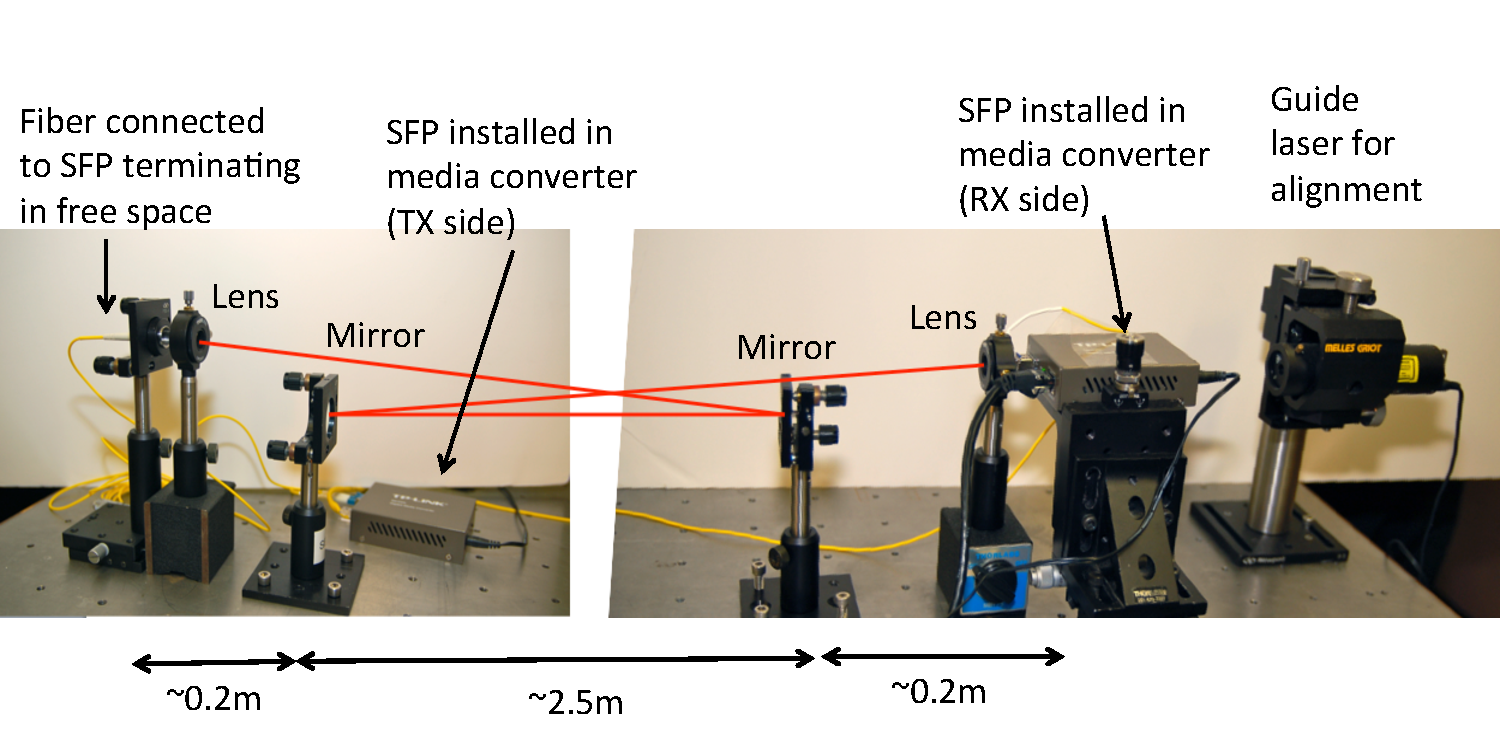
\includegraphics[width=250pt]{PPTFigs/complete-optical-setup-fig.pdf} 
%\vspace{-0.8in}
} 
\hspace*{0.3in}
\subfloat[Throughput stability]
{
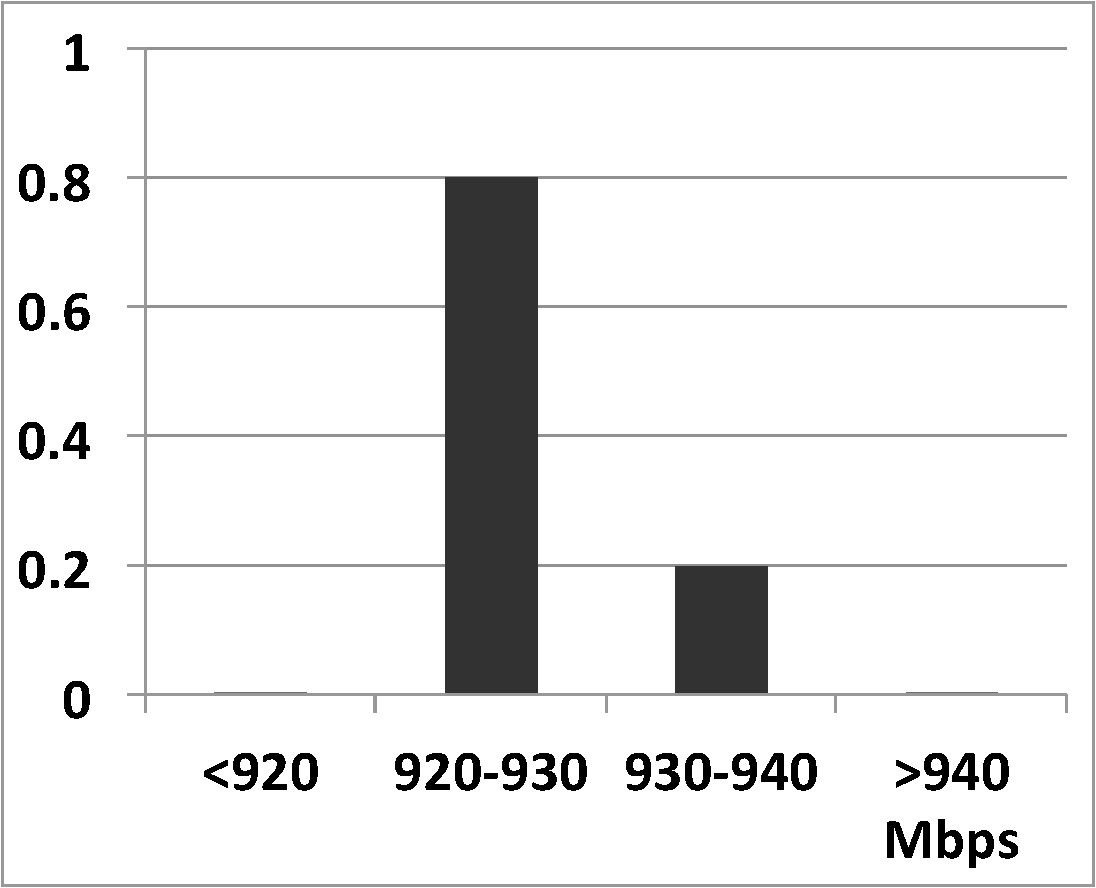
\includegraphics[width=100pt]{Figures/link-thrpt.pdf} 
}
\caption{(a) Experimental prototype showing FSO communication using SFP over ~7.5m.
Note use of mirrors to achieve a long beam path on a standard size optical bench. (The beam is hand drawn.) 
(b) Distribution
of per-second TCP throughputs (in Mbps) over a continuous 30 hour period over ~7.5m.}
\label{fig:optics-layout}
%\end{wrapfigure}
\end{figure}

\para{Preliminary Demonstration of Feasibility.}  We have developed a
proof-of-concept prototype to demonstrate feasibility of designing
FSOs from optical SFPs. See Figure~\ref{fig:optics-layout}. The
prototype uses a pair of 1Gbps SFPs using 1310nm lasers.  We launch
the beam from a single-mode optical fiber connected to the TX SFP on
one end \blue{with the other end terminating in free space.} Due to
the narrow $8-10 \mu\mbox{m}$ fiber diameter, the initial beam
divergence is very large. We used an achromatic doublet lens to
collimate the beam to a roughly 4mm diameter waist with the fiber tip
positioned at the focal point of the lens. (An optical bench and
translating mounts help in the positioning.) The collimated beam
propagates to a distance of 7.5m where an identical lens re-focuses
beam on the RX detector.\footnote{Since the SFP used here uses two
  separate optical paths (for duplex operation), the return link is
  closed using a regular fiber.} We connect the SFPs to a laptop each
via standard media converters~\cite{} and run TCP throughput
experiments for 30 hours to test link stability.
Figure~\ref{fig:optics-layout} demonstrates very stable link
performance comparable to the wired case. We also analyzed the
sensitivitity of our prototype to misalignment between the TX-RX and
found that the throughput is stable up to a transverse shift of
$\pm0.7 mm$.

\subsection{Precise and Fast Beam Redirection}

\begin{task}
\blue{Develop fast and effective beam path redirection techniques to achieve 
reconfiguration in the interconnection fabric.}
\end{task}

\smallskip

% DD, Survey
The result of the previous investigation will provide the basis for a
high-speed reliable link, but we still need a {\em beam steering
  mechanism}.  A wide spectrum of candidate solutions exist for laser
beam steering including phased array techniques~\cite{}. But most of
these are not commodity and some are subjects of active
research. Feasibility and cost-effectiveness for adapting these
solutions for DCs are unknown. For feasibility reasons, we have
investigated two candidate commodity technologies that we will
describe in this section.
% TWO TIMESCALES
Irrespective of the technology used,  there are two fundamental granularities
of  beam ``movements'':

\begin{packedenumerate}
\item{\em Steering:} This refers to the central mechanism where a FSO
  beam emanating from a TX is redirected to a different RX. This must
  be done at a fast time scale -- few millseconds in order to be
  responsive to DC traffic dynamics.  Physical and optical
  limitations, however, induce constraints such that each transceiver
  may only be able to link to only a {\em subset} of other
  transceivers in the DC.  The specific types of constraints may be
  technology-specific as we will see later.

\item {\em Pre-configuration:} Given the above constraint, the above
  subset has to be chosen in a semi-offline fashion for each FSO
  transceiver independently. This gives rise to interesting topology
  design problems that we address in Section~\ref{sec:topology}.
\end{packedenumerate}

%% SCOPE THE WORK
%First we describe the proposed 
%\Preconfiguration can be done simply by using servos that orient 
%specific components to a pre-determineed
%As such, developing a 
%complete solution 
%the \Preconfiguration is outside the scope of the project.

In our proposed research, we will investigate two promising steering
mechanisms, with different tradeoffs as discussed below.

\para{Switchable Mirrors.} Switchable mirrors (SMs) are made from a
special liquid crystal material that can be electrically controlled to
rapidly switch between reflection (mirror) and transparent (glass)
states at millisecond timescales~\cite{sm}. These are used in various
forms of visual aids in niche markets e.g., rear-view video mirror.
Figure~\ref{fig:beam-redirect}(a) conceptually shows how we can use
SMs for beam redirection.  Each FSO device will be equipped with
multiple SMs, with each SM pre-aligned (offline; part of
pre-configuration) to a dedicated beam path. The desired link is
established by swithcing one of the SMs on the TX in the mirror state
and the other SMs in the transparent state. (An analogous arrangement
will be made at the other end, but not shown for ease of
visualization.)  As mentioned earlier, the ceiling mirror redirects
the beam back to the receiving rack, making efficient use of the
above-rack space while minimizing interference. When manufactured at
scale, each small-size SM will have minimal cost ($<$
\$5~\cite{sm-personal}).

\softpara{Preliminary Study.} We evaluated the viability of switchable
mirrors~\cite{hotnets} using a 12" x 15" switchable mirror (SM) from
Kentoptronics~\cite{sm} tuned for the IR spectrum. The switching
latency of the SM is found to be around 250 msec. Because the
switching latency is proportional to the SM’s surface
area~\cite{sm-size}, we estimate a $<5$ msec latency for a small (1" x
1") SM we propose to use. Finally, we confirmed that the FSO beam can
be reflected from conventional mirrors with no loss in TCP throughput
even after multiple reflections.

\begin{figure*}[t] %{r}{0.5\textwidth}
\centering
\subfloat[SM: In the top-half the second SM is in mirror mode,
redirecting the beam to Receiver 1, while the bottom half has SM3 in
 mirror mode and thus redirecting to Receiver 2.]
{
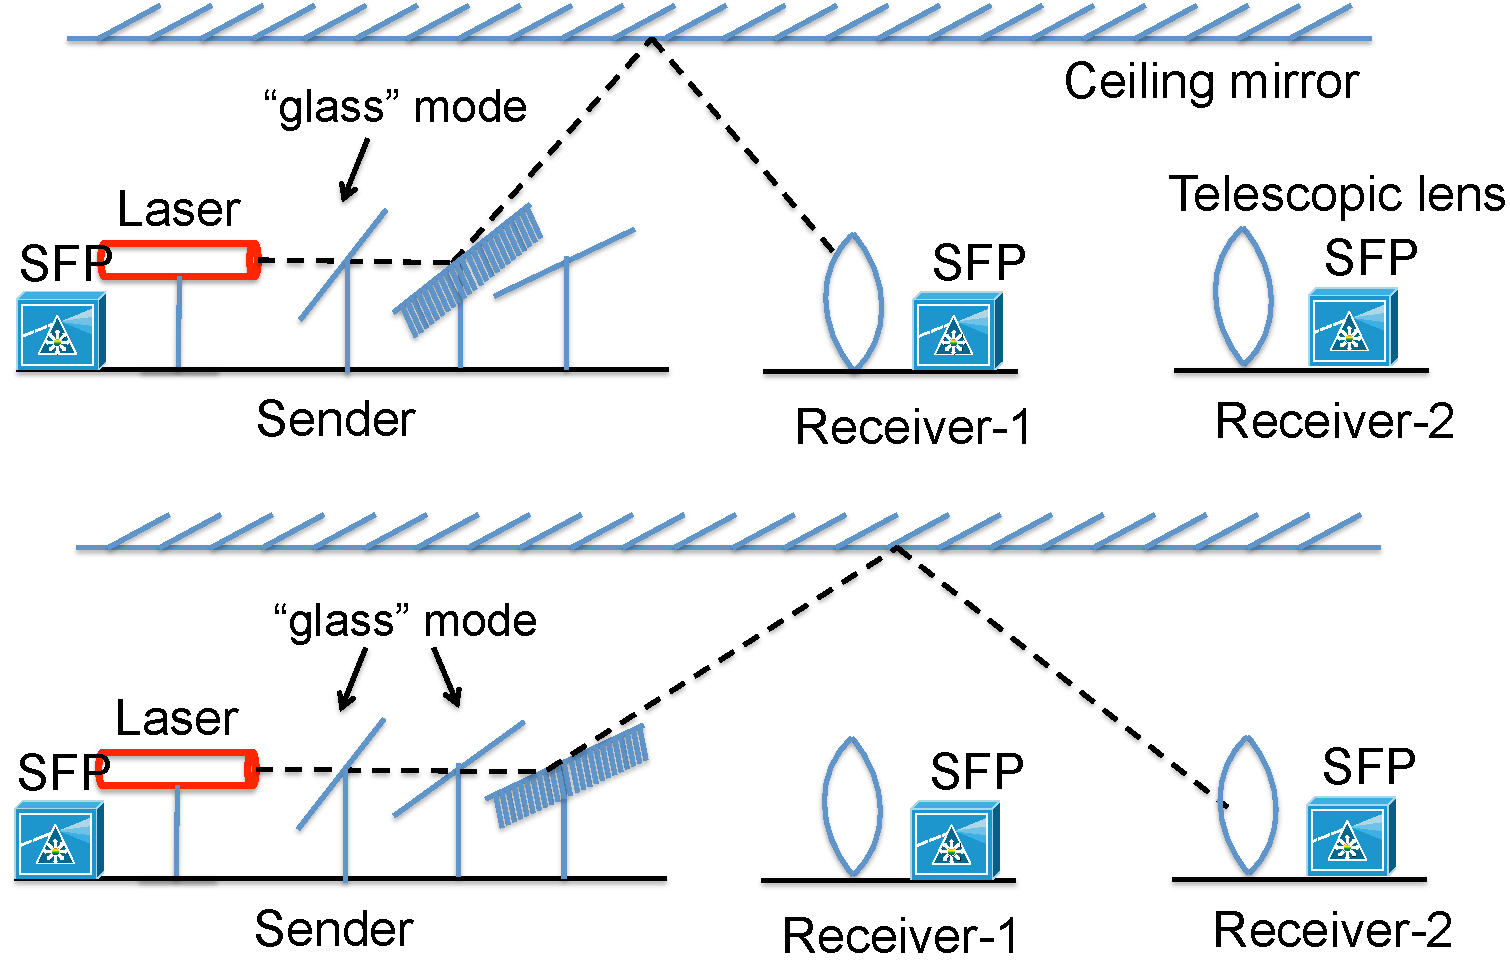
\includegraphics[width=150pt]{Figures/SM-fig.pdf} 
}
\hspace{1cm}
\subfloat[GM: Two mirrors direct incident beam into a rectangular cone. ]
{
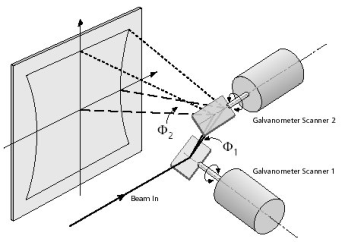
\includegraphics[width=130pt]{Figures/GM-fig.pdf} 
}
\caption{Candidate beam re-direction approaches.}
\label{fig:beam-redirect}
\end{figure*}

\para{Galvo Mirrors.} A Galvo mirror (GMs)~\cite{} is basically a
Galvanometer in principle, except that instead of moving a pointer in
response to current, it moves a small mirror.  GMs are conventionally
used in various laser scanning applications -- both precision
industrial as well as infotainment like laser shows.  As shown in
Figure~\ref{fig:beam-redirect}(b), two computer-controlled, motorized
mirrors are mounted at right angles direct the incident beam into a
rectangular cone.  The (fixed) incident beam can thus be directed into
a rectangular cone under computer control.  Commercially available
systems~\cite{} can provide a cone half angle ($\Phi_1$ and $\Phi_2$)
of $\pm 20^\circ$, for a total rectangular cone angle of $40^\circ$ in
both directions.  A typical pointing accuracy is within 15
$\mu$rad~\cite{}, resulting in a beam positioning precision within
1.5mm for beam paths of up to 100m. Typical steering latency is
\plsfill. \blue{Something about MEMs here.}

\cbl 
\softpara{Custom Building a Small and Inexpensive GM.} Commodity GM
assemblies are expensive (\$ 2000) and much larger than we desire due
to the associated machinary.  One way to minimize the space used on
the rack is to keep only the optical components on the top of rack,
and hide the motor and associated electronics underneath the rack
(using use custom designed extension arms to hold the mirrors) But
additional stability and precision issues must be addressed.  \cb

\para{SM vs.\ GM Tradeoff.}  The key difference between the two
steering mechanisms is the topological possibilites they yield: a GM
can reach {\em any} receiver within the \blue{prescribed} cone (of
limited angle), while use of $\NumSMsPerFSO$ SMs with an FSO provides
$k$ {\em arbitrary} target receivers. Use of GM may obviate the need
for additional alignment (e.g., piezo electric positioners), but
commodity GM assemblies are much larger than we desire due to the
associated machinary. In our research, we will systematically
investigate the impact of these tradeoffs, and use a hybrid
architecture consisting of both steering mechanisms.

\para{Pre-configuration Machinery.} Note that SMs and GMs will need to
be aligned (or oriented), to target the desired set of
receivers. However, this is done in a semi-offline fashion, so speed
is not of the essence. In particular, the desired alignments can be
pre-computed and achieved by servos that simply orient the attached
component (e.g., SM, GM) to the desired position. Micro adjustments
can be done using the piezo-electric positioners described before. We
skip further details of the above pre-configuration machinery since it
is outside the scope of this project. However, we discuss
pre-configured topology design challenges in the next section.

\hg{I removed the ``overall cost'' para; I think its unnecessary, and
  can instead go in {\em budget justification}.}  








